\documentclass[12pt, twoside]{article}
\usepackage[letterpaper, margin=1in, headsep=0.2in]{geometry}
\setlength{\headheight}{0.6in}
%\usepackage[english]{babel}
\usepackage[utf8]{inputenc}
\usepackage{microtype}
\usepackage{amsmath}
\usepackage{amssymb}
%\usepackage{amsfonts}
\usepackage{siunitx} %units in math. eg 20\milli\meter
\usepackage{yhmath} % for arcs, overparenth command
\usepackage{tikz} %graphics
\usetikzlibrary{quotes, angles}
\usepackage{graphicx} %consider setting \graphicspath{{images/}}
\usepackage{parskip} %no paragraph indent
\usepackage{enumitem}
\usepackage{multicol}
\usepackage{venndiagram}

\usepackage{fancyhdr}
\pagestyle{fancy}
\fancyhf{}
\renewcommand{\headrulewidth}{0pt} % disable the underline of the header
\raggedbottom
\hfuzz=2mm %suppresses overfull box warnings

\usepackage{hyperref}

\fancyhead[LE]{\thepage}
\fancyhead[RO]{\thepage \\ Name: \hspace{4cm} \,\\}
\fancyhead[LO]{BECA / Dr. Huson / Geometry\\*  Unit 2: Angles\\* 4 October 2022}

\begin{document}

\subsubsection*{2.2 Extension: Clock problems}
\begin{enumerate}[itemsep=0.5cm]
\item A clock face is shown with both hands vertical, pointing at the 12, indicating 12:00. 
\begin{enumerate}
  \item Draw the positions of the minute and hour hands at 3:00 on the second clock.
  \item What angle is made by the two hands at 3:00?
\end{enumerate}
  \begin{tikzpicture}
    \draw (0,0) circle [radius=2];
    \draw (0,0) circle [radius=0.1];
    \foreach \x in {1,...,12}
      \node at ({90+\x*-30}:1.8){\x};
      \draw[->, ultra thick] (0,0)--(90:1);
      \draw[->, gray] (0,0)--(90:1.5);
    %\draw[->,thick] (0,0)--(-30:1.5);
    \draw[->,dashed] (90:0.5) arc (90:-30:0.5);
    %\draw[->,thick,red] (0,0)--(-60:1.5);
    %\draw[->,thick,red] (0,0)--(-180:1.5);
    %\draw[->,dashed,red] (-60:1) arc (-60:-180:1);
  \end{tikzpicture} \hspace{2cm}
  \begin{tikzpicture}
    \draw (0,0) circle [radius=2];
    \draw (0,0) circle [radius=0.1];
    \foreach \x in {1,...,12}
      \node at ({90+\x*-30}:1.8){\x};
  \end{tikzpicture}

\item How many degrees does the minute hand move in an hour?
\item How many degrees does the hour hand move in an hour?
\item How many minutes does it take the minute hand to move 90 degrees?
\item How many minutes does it take the hour hand to move 90 degrees? 
\item Write an expression to model the angle measure the minute hand makes versus vertical after $t$ minutes. \vspace{0.5cm}

\item Mark the positions of the minute and hour hands at 3:30. What angle is made now? \par \vspace{0.5cm}
  \begin{tikzpicture}
    \draw (0,0) circle [radius=2];
    \draw (0,0) circle [radius=0.1];
    \foreach \x in {1,...,12}
      \node at ({90+\x*-30}:1.8){\x};
  \end{tikzpicture}


\newpage
\item Two supplementary angles have measures m$\angle ABD = 2x$ and m$\angle DBC = 4x + 60^\circ$. \\[0.25cm] 
  Write an equation, then find $x$. \vspace{0.5cm}
    \begin{flushright}
      \begin{tikzpicture}[scale=1]
        \draw[<->, thick]
          (0:5) coordinate (a) node[below left] {$C$}
          -- (0,0) coordinate (b) node[below] {$B$}
          -- (125:3) coordinate (c) node[above right] {$D$}
          pic["$4x+60^\circ$", <->, draw=black, angle eccentricity=1.5, angle radius=1cm]
          {angle=a--b--c};
          \draw[<-, thick]
          (180:4) coordinate (d) node[below] {$A$}
          -- (0,0) coordinate (e)
          pic["$2x$", <->, draw=black, angle eccentricity=1.5, angle radius=1cm]
          {angle=c--e--d};
      \end{tikzpicture}
    \end{flushright}
      
\item Given the perpendicular situation shown, $\overrightarrow{BD} \perp \overleftrightarrow{ABC}$ and angle measures given. \\[0.25cm] 
  Find $x$. \vspace{0.25cm}
    \begin{multicols}{2}
      m$\angle DBE = 35^\circ$ \\[0.25cm]
      m$\angle EBC = 3x + 10^\circ$ \\[0.25cm]
      \begin{tikzpicture}[scale=1]
        \draw[<->, thick]
          (0:5) coordinate (a) node[below left] {$C$}
          -- (0,0) coordinate (b) node[below] {$B$}
          -- (50:5) coordinate (c) node[below right] {$E$}
          pic["$3x + 10$", <->, draw=black, angle eccentricity=2, angle radius=1cm]
          {angle=a--b--c};
          \draw[<-, thick]
          (90:4) coordinate (d) node[right] {$D$}
          -- (0,0) coordinate (e)
          pic["$35^\circ$", <->, draw=black, angle eccentricity=1.5, angle radius=1cm]
          {angle=c--e--d};
          \draw[->, thick] (0,0)--(-180:2) node[below right]{$A$};
          \draw (0,0)++(-0.3,0)--++(0,0.3)--+(0.3,0);
      \end{tikzpicture}
    \end{multicols} \vspace{1cm}

\item The perimeter of the isosceles $\triangle FGH$ is 115 and $\overline{FH} \cong \overline{GH}$. Given $FG=5x+16$ and $FH=34 \frac{1}{2}$. \\[0.25cm]
Write an equation to find $x$, then solve and check.\\[0.25cm]
  \begin{tikzpicture}[scale=0.5]
    \draw[thick](0,0)--(8,0)--(4,4)--(0,0);
    \draw[fill] (0,0) circle [radius=0.05] node[below left]{$F$};
    \draw[fill] (8,0) circle [radius=0.05] node[below right]{$G$};
    \draw[fill] (4,4) circle [radius=0.05] node[above right]{$H$};
    \draw[thick] (1.8,2.3)--(2.4,1.9); %tick mark
    \draw[thick] (5.6,1.9)--(6.2,2.3); %tick mark
    \node at (4,0) [below]{$5x+16$};
    \node at (1.6,3) [left]{$34 \frac{1}{2}$};
  \end{tikzpicture}
  
\end{enumerate}
\end{document}